\begin{figure}[h]
    \centering
    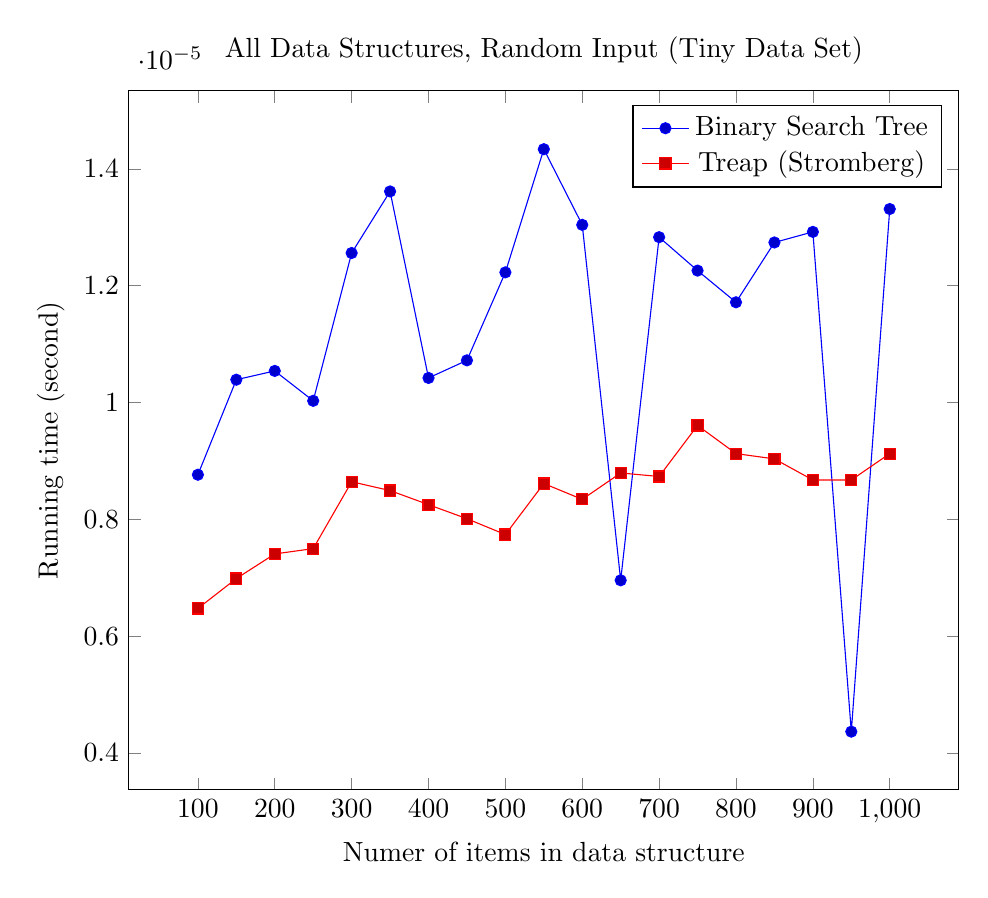
\begin{tikzpicture}
        \begin{axis}[
            xlabel={Numer of items in data structure},
            ylabel={Running time (second)},
            title={All Data Structures, Random Input (Tiny Data Set)},
            width=\textwidth
        ]
		\addplot coordinates {
			(100, 8.764202299449408e-06)
			(150, 1.0390549117911263e-05)
			(200, 1.0541136786290651e-05)
			(250, 1.0029138713818498e-05)
			(300, 1.2559011542556674e-05)
			(350, 1.3613125221167977e-05)
			(400, 1.0420666651622667e-05)
			(450, 1.0721841988337033e-05)
			(500, 1.2227718672130905e-05)
			(550, 1.4335946029353509e-05)
			(600, 1.3040892081361832e-05)
			(650, 6.957150278941171e-06)
			(700, 1.2830069345648453e-05)
			(750, 1.2257836205797901e-05)
			(800, 1.1715720599658752e-05)
			(850, 1.2739716744603059e-05)
			(900, 1.2920421946649441e-05)
			(950, 4.367042382913411e-06)
			(1000, 1.331194988445361e-05)
		};
		\addplot coordinates {
			(100, 6.475269740180423e-06)
			(150, 6.987267812608167e-06)
			(200, 7.408913284079333e-06)
			(250, 7.499265885080319e-06)
			(300, 8.643732164781426e-06)
			(350, 8.493144496402038e-06)
			(400, 8.252204226977255e-06)
			(450, 8.01126395759688e-06)
			(500, 7.740206154549512e-06)
			(550, 8.613614631070022e-06)
			(600, 8.342556828022651e-06)
			(650, 8.794319833160813e-06)
			(700, 8.734084765826822e-06)
			(750, 9.60749324239174e-06)
			(800, 9.125612703586583e-06)
			(850, 9.035260102541187e-06)
			(900, 8.673849698448422e-06)
			(950, 8.673849698448422e-06)
			(1000, 9.125612703542173e-06)
		};
        \legend{Binary Search Tree, Treap (Stromberg)}
        \end{axis}
    \end{tikzpicture}
    \caption{Average of 10 operations, benchmarked every 50, starting at 100.}
\end{figure}